\documentclass{article}

% Encoding
\usepackage[utf8]{inputenc}
% Little tweaks for the margins
\usepackage[margin=2.5cm]{geometry}
% Including graphics
\usepackage{graphicx}

\title{LINFO1252 : Système Informatique}
\author{Nathan Tihon}
\date{\today}

\title{LINFO1252 : Système Informatique}
\author{Nathan Tihon}
\date{\today}

\begin{document}

\maketitle
\newpage

\section{Introduction}

Le but de ce projet est d'implémenter et évaluer les performances de plusieurs algorithmes de synchronisations.
L'évaluation de performances s'articule autour de 2 paramètres, le nombre de \textit{thread} (paramètre entier) et le type de primitive de synchronisation utilisées (paramètre catégoriel).
Le nombre de thread sera un entier compris entre 1 et $2n$ où $n$ est le nombre de coeurs du processeur utilisé.
Les primitives utilisées appartiendront quant à elle à 2 catégories, la première comprendra les mutex et sémaphores POSIX de la librairie standard tandis que la seconde incluera les verrous à attente active ainsi que les sémaphores construites sur ces verrous.
Les figures analysées dans ce rapport suivent toutes le même schéma, elles sont composées de deux sous-graphe comprenant chacun deux couleurs.
Le sous-graphe supérieur comprend une moyenne du temps d'exécution en fonction des paramètres tandis que le sous-graphe inférieur représente l'écart-type dans les même conditions.
Les couleurs représentent la catégorie de primitives utilisées (paramètre catégoriel), l'axe des abscisses montre le nombre de thread (paramètre entier) et l'axe des orconnées représente le temps d'exécution en fonction de ces paramètres.

\section{Verrous à attente active}

La figure ci-dessous représente les performances des verrous à attente active. 
Les deux couleurs permettent de montrer l'algorithme utilisé. 
Le bleu représente l'utilisation de l'algorithme \textit{test-and-set} alors que le jaune représente l'utilisation de l'algorithme \textit{test-and-test-and-set}.\footnote{Par simplicité, je me réfèrerai à ces 2 algorithmes par TAS et TATAS}

\begin{figure}[h!]
    \centering
    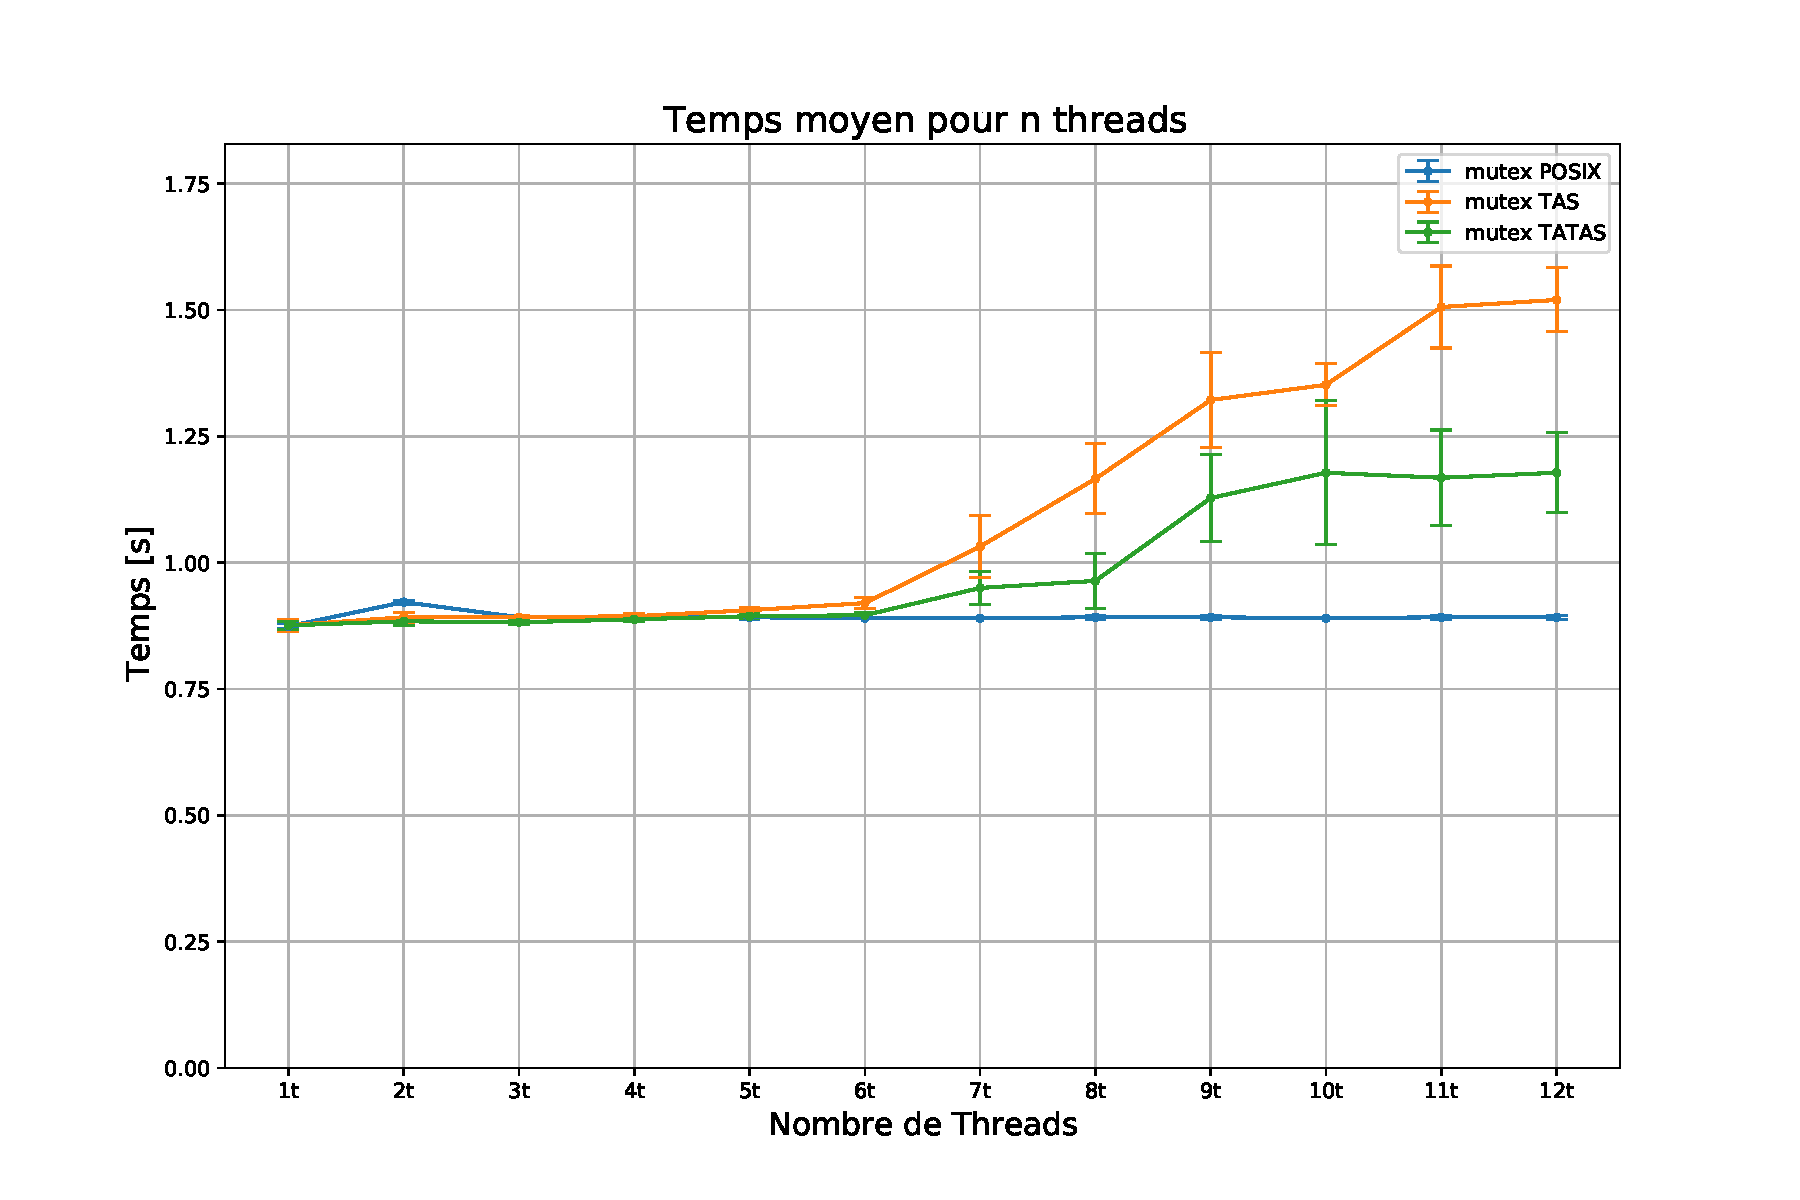
\includegraphics[scale=0.5]{img/spinlock.pdf}
    \caption{Temps d'exécution d'un verrou à attente active dans différentes conditions}
    \label{pic:spinlock}
\end{figure}

Nous pouvons observer que les performances sont assez semblables jusqu'à atteindre un seuil de 6 threads, seuil à partir duquel les performances divergent.
On peut ensuite observer que l'algorithme TATAS performe bien mieux que le TAS, allant parfois jusqu'à un speedup de 50\%. 
Cela peut être expliqué par le fait que l'algorithme TAS, effectue des blocages répétés du bus de cache (à cause de l'instruction \texttt{xchg}) ce qui ralentit considérablement la vitesse à laquelle les différents coeurs synchronisent leur cache (et donc les variables partagées).

\section{Problème des philosophes}

\begin{figure}[h!]
    \centering
    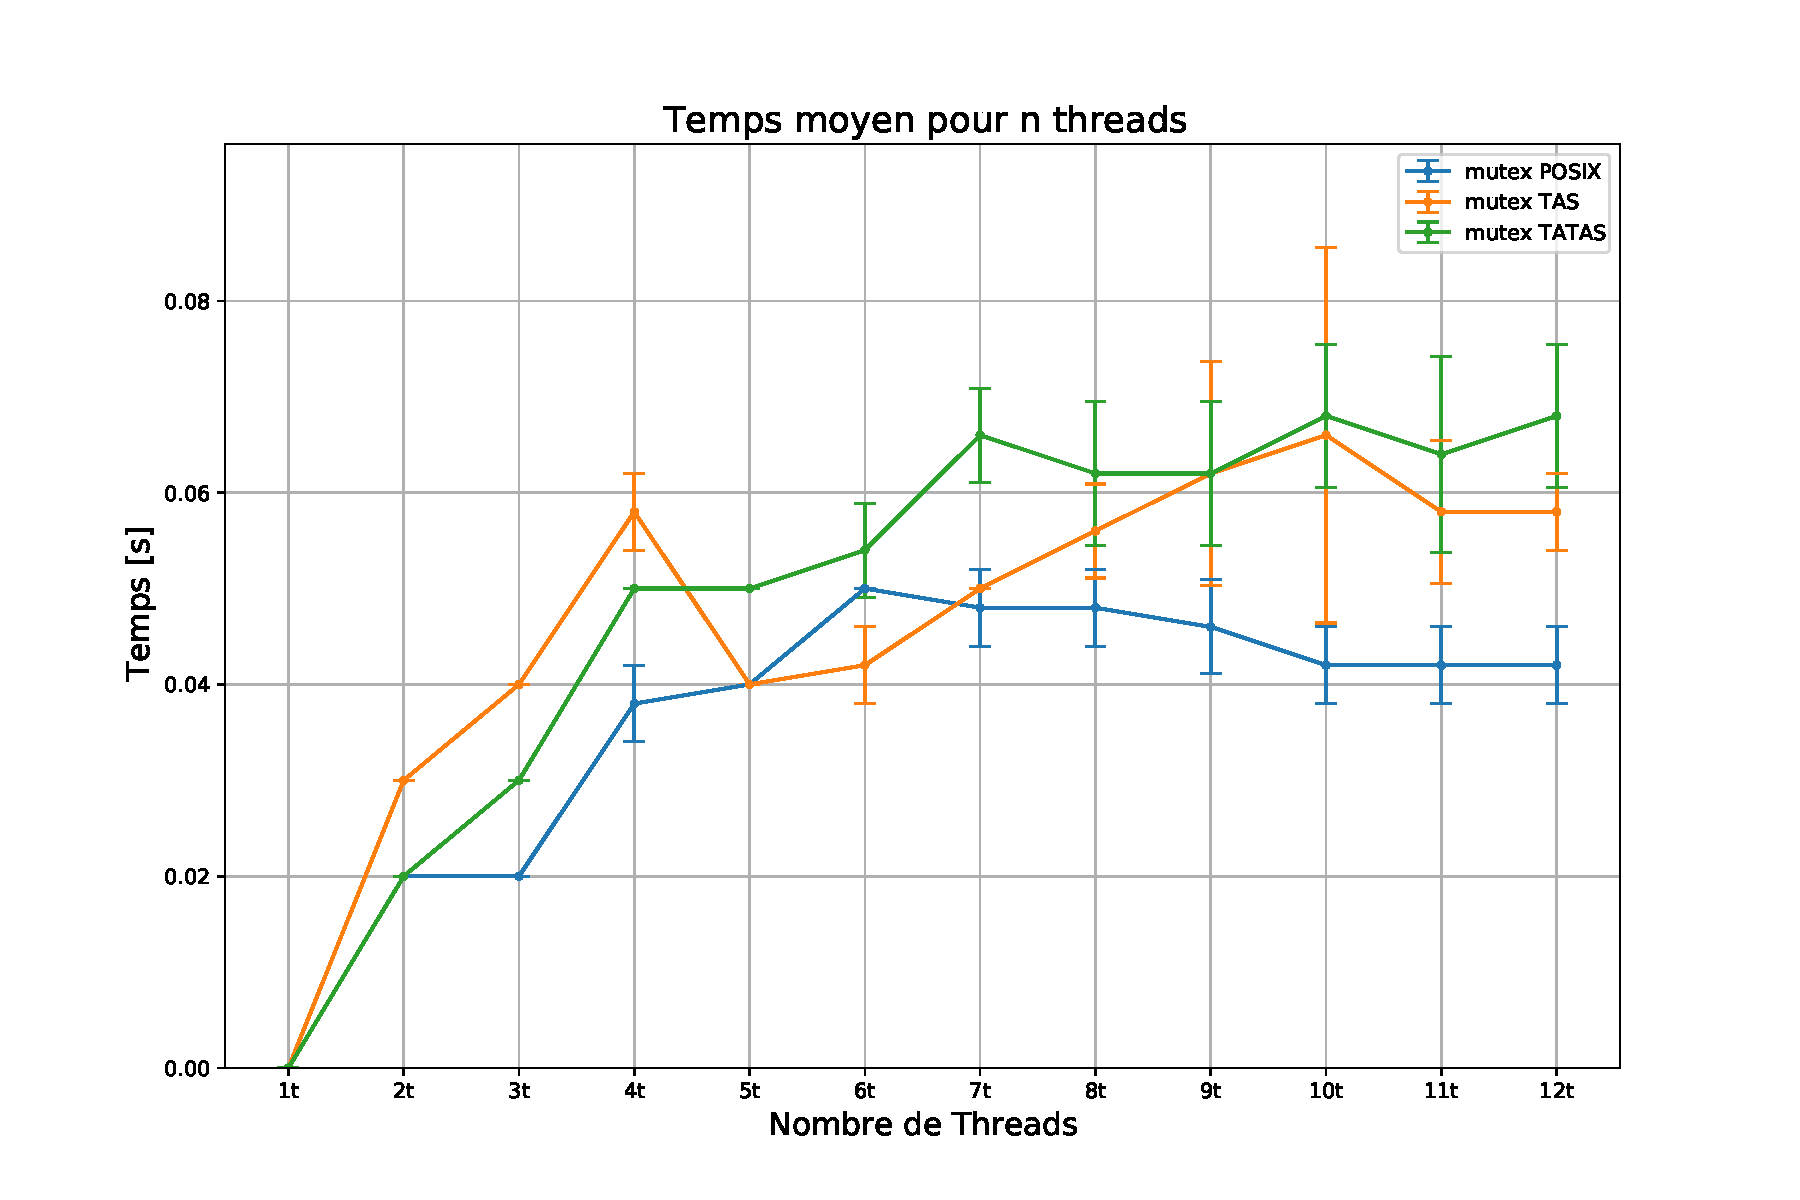
\includegraphics[scale=0.5]{img/philosophes.pdf}
    \caption{Temps d'exécution du problème des philosophes dans différentes conditions}
    \label{pic:philo}
\end{figure}


\section{Problème des Producteurs-Consommateurs}


\begin{figure}[h!]
    \centering
    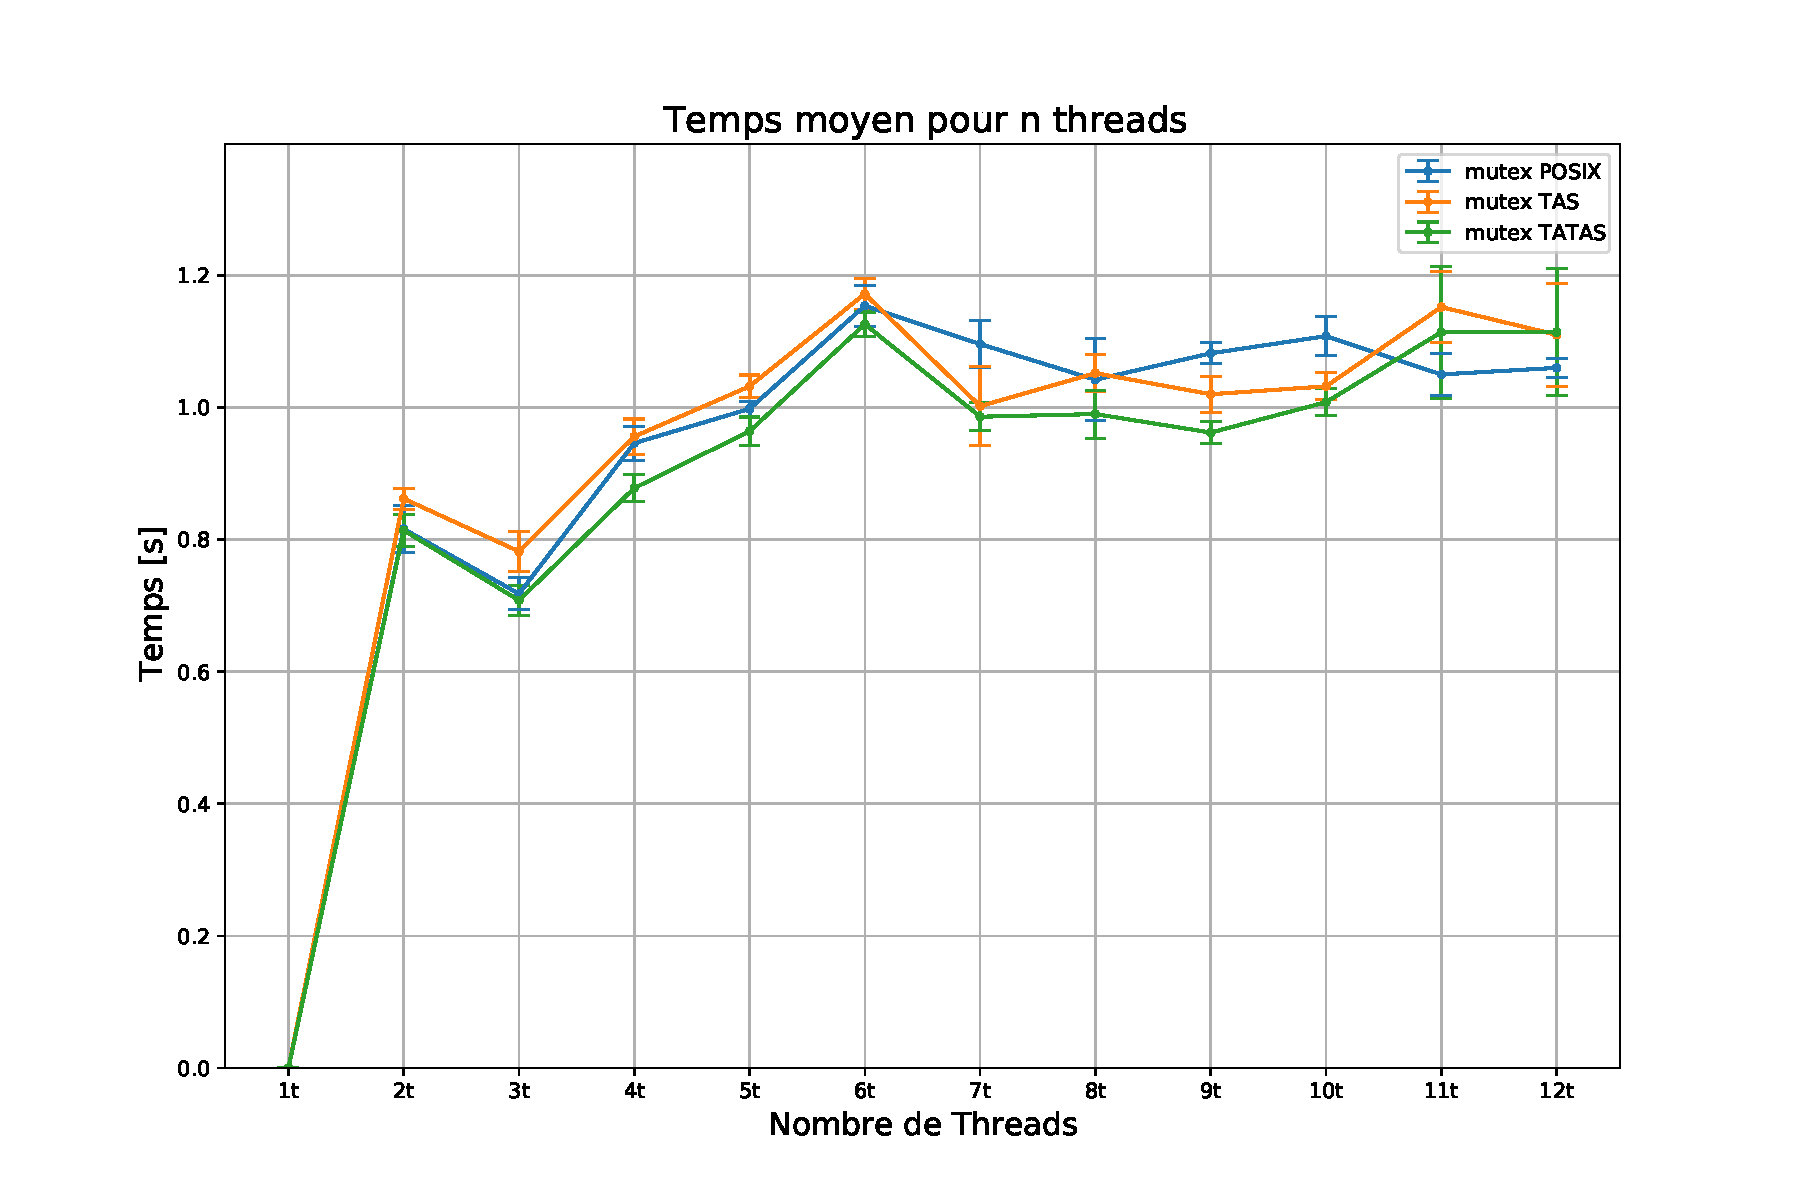
\includegraphics[scale=0.5]{img/prodcons.pdf}
    \caption{Temps d'exécution du problème des producteurs-consommateurs dans différentes conditions}
    \label{pic:prodcons}
\end{figure}


\section{Problème des lecteurs-écrivains}

\begin{figure}[h!]
    \centering
    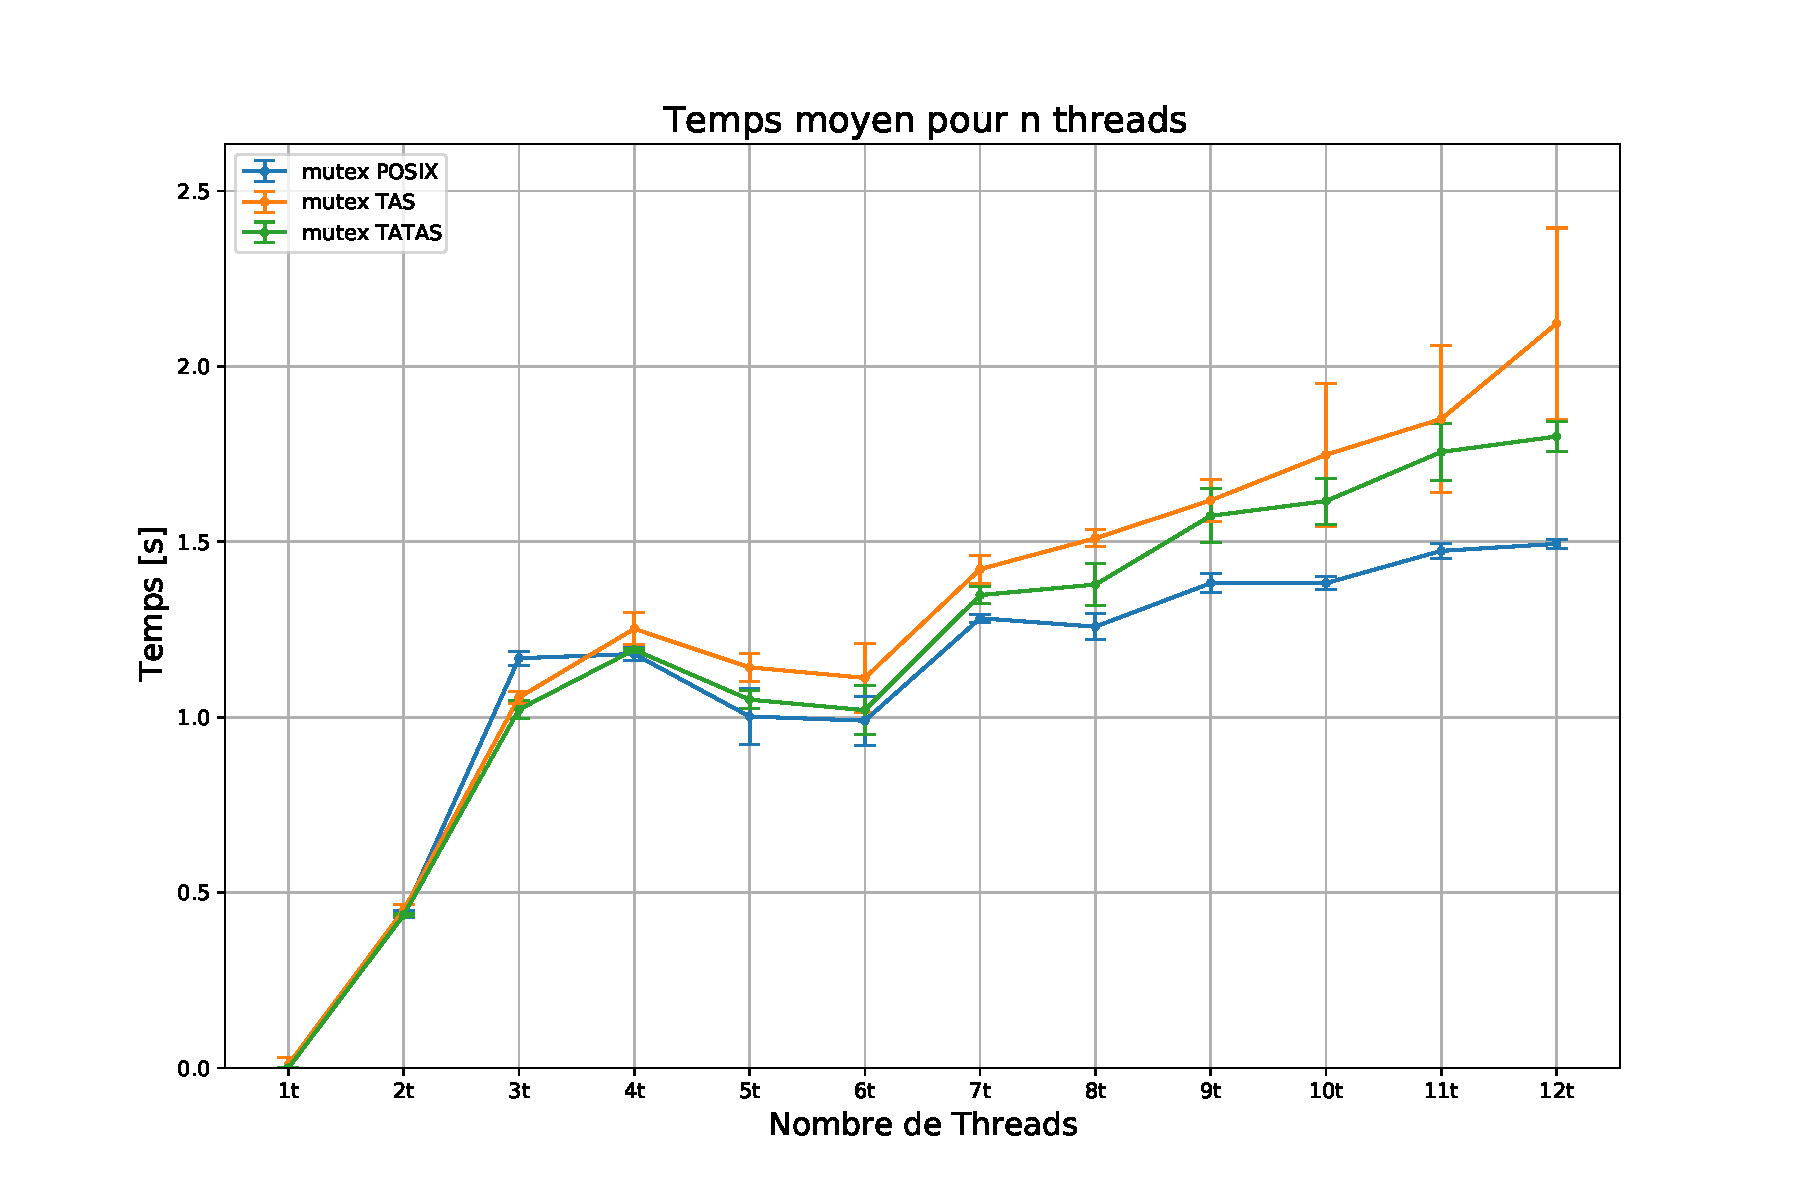
\includegraphics[scale=0.5]{img/readwrt.pdf}
    \caption{Temps d'exécution du problème des lecteurs-écrivains dans différentes conditions}
    \label{pic:readwrt}
\end{figure}

\end{document}